

\section{Automatisches Wechseln von Differenzialgleichungslösern}

Im Kapitel \ref{sec:numerisches_lösen_von_anfangswert_problemen} wurde das implizite mit dem expliziten Euler-Verfahren miteinander verglichen.
In diesem Kapitel wird untersuch, wie die Vorteile beider Verfahren so miteinander verbunden 
werden können, dass das Projekt sowohl mit einer hohen Genauigkeit, als auch einer verträglichen Laufzeit
ausgeführt werden kann.
Wie bereits gezeigt wurde, liefern die unterschiedlichen Löser zu unterschiedlichen Zeitpunkten
unterschiedlich gute Ergebnisse.
Das \textit{DifferentialEquations.jl} Projekt bietet dafür die Möglichkeit, automatisch 
zwischen verschiedenen Lösungsverfahren zu wechseln.
Dies geschieht meist abhängig von aktuellen Fehler, es können aber auch eigene Kriterien entwickelt werden.
Dabei ist jedoch zu beachten, dass dies nicht mit allen Verfahren möglich ist.
So ist es zum Beispiel nicht möglich, den impliziten mit dem expliziten Euler zu verbinden.
Deshalb wird im folgendem der \textit{Tsit5} mit dem \textit{Rosenbrock23} verbunden. Dieser Algorithmus wird im folgendem als AutoTsit5 bezeichnet.
Dessen Laufzeit kann stark variieren. Je nach Problem kann die Laufzeit zwischen ein paar Sekunden und
ein paar Stunden sein.
In den für dieses Kapitel berechneten Trajektorien, war die geringste Laufzeit 19 Sekunden und die längste 2 Stunden.
Die genaue Laufzeit hängt sehr stark von den benötigten Fehlertoleranzen und der Problemgröße ab.
Im Folgenden wird das bereits genannte Verfahren mit dem expliziten Euler verglichen.

In der Grafik \ref{fig:vergleichexplizit} wird die Differenz zwischen dem expliziten Euler-Verfahren und dem \textit{AutoTsit5} verglichen.
In den ersten 0,5 Sekunden ist die Differenz positiv, dies bedeutet, dass
der explizite Euler bessert.
Danach liefert der \textit{AutoTsit5} dann ein konstant besseres Ergebnis.

In der Graphik \ref{fig:vergleichimplizit} wird beobachtet,
dass der \textit{AutoTsit5} am Anfang ein besseres Ergebnis liefert.
Nach etwa 1 Sekunde wird dann der implizite Euler besser.
Besonders ist vor allem, dass der Unterschiede zwischen beiden Verfahren gegen Ende sich sehr stark null annähert und bei zwei der drei Trajektorien gegen Ende  der \textit{AutoTsit5} wieder ein besseres Ergebnis liefert.

Daraus lässt sich folgern, dass die automatischen Verfahren bei längeren Trajektorien ein leicht besseres Ergebnis liefern.

Dies liegt vermutlich daran, das diese die Vorteile von 
zwei verschiedenen Lösungsverfahren ausnutzen können.

\begin{figure}[H]
    \centering
    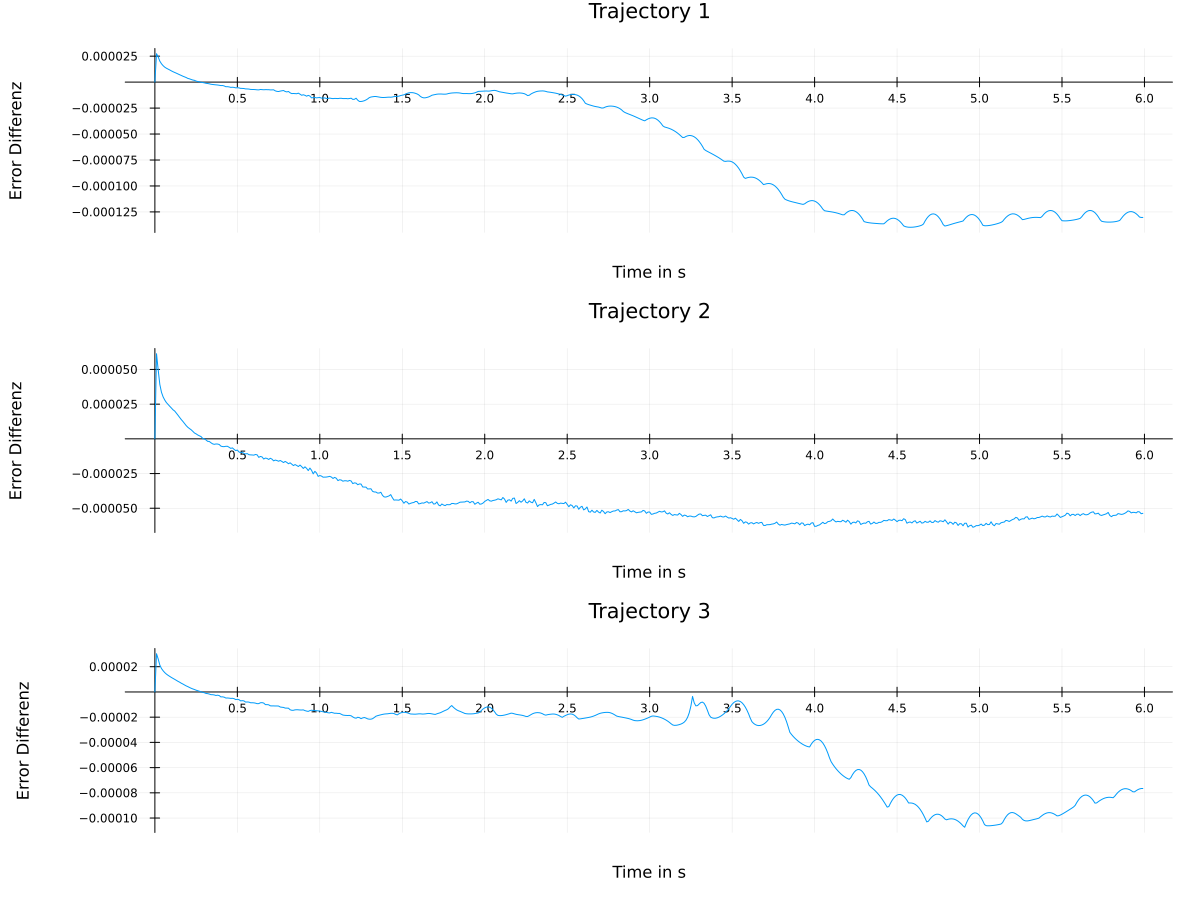
\includegraphics[width=0.8\textwidth]{Data/03_Ergebnisse/autoswitching/errors_explizit_composit.png}
    \caption{Vergleich mit dem expliziten Algorithmus}
    \label{fig:vergleichexplizit}
\end{figure}
\begin{figure}[H]
    \centering
    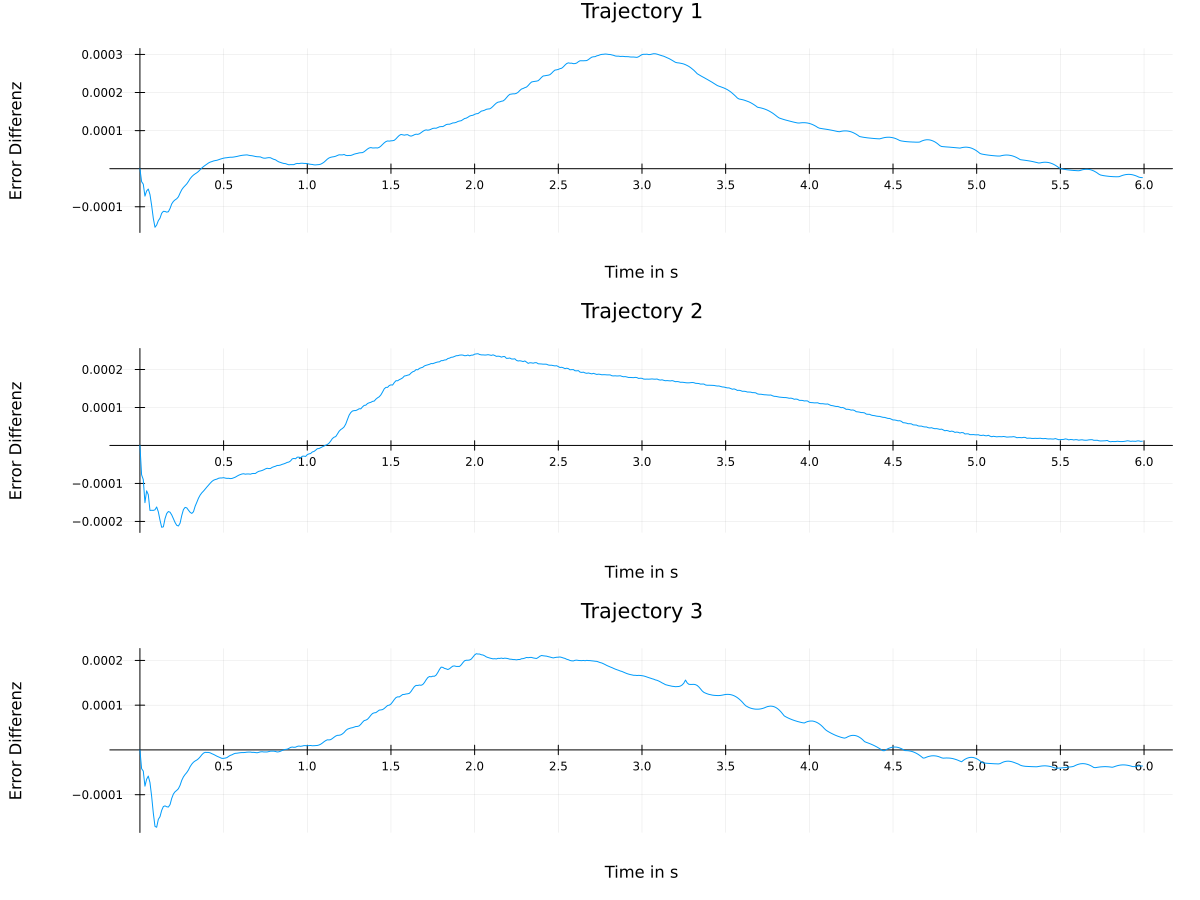
\includegraphics[width=0.8\textwidth]{Data/03_Ergebnisse/autoswitching/errors_implizit_composit.png}
    \caption{Vergleich mit dem impliziten Algorithmus}
    \label{fig:vergleichimplizit}
\end{figure}

